\documentclass[aspectratio=169,11pt]{beamer}

% ---------- Theme Colors (matching ELTE-style design) ----------
\definecolor{UNBBlue}{RGB}{0,40,85}
\definecolor{UNBLightBlue}{RGB}{100,150,200}
\definecolor{UNBGray}{RGB}{128,128,128}
\definecolor{UNBLightGray}{RGB}{240,240,240}
\definecolor{UNBGreen}{RGB}{39,174,96}
\definecolor{UNBRed}{RGB}{231,76,60}
\definecolor{UNBOrange}{RGB}{243,156,18}

% ---------- Theme Configuration ----------
\usetheme{Madrid}
\usecolortheme{default}

% Color Customization
\setbeamercolor{palette primary}{bg=UNBBlue,fg=white}
\setbeamercolor{palette secondary}{bg=UNBLightBlue,fg=white}
\setbeamercolor{palette tertiary}{bg=UNBBlue,fg=white}
\setbeamercolor{palette quaternary}{bg=UNBBlue,fg=white}
\setbeamercolor{structure}{fg=UNBBlue}
\setbeamercolor{frametitle}{bg=UNBBlue,fg=white}
\setbeamercolor{title}{bg=UNBBlue,fg=white}
\setbeamercolor{block title}{bg=UNBBlue,fg=white}
\setbeamercolor{block body}{bg=UNBLightGray,fg=black}

% Font Settings
\setbeamerfont{title}{size=\Large,series=\bfseries}
\setbeamerfont{frametitle}{size=\large,series=\bfseries}
\setbeamerfont{block title}{size=\normalsize,series=\bfseries}

% Remove navigation symbols
\setbeamertemplate{navigation symbols}{}

% Custom footer
\setbeamertemplate{footline}{
  \leavevmode%
  \hbox{%
    \begin{beamercolorbox}[wd=.3\paperwidth,ht=2.25ex,dp=1ex,center]{author in head/foot}%
      \usebeamerfont{author in head/foot}\insertshortauthor
    \end{beamercolorbox}%
    \begin{beamercolorbox}[wd=.4\paperwidth,ht=2.25ex,dp=1ex,center]{title in head/foot}%
      \usebeamerfont{title in head/foot}\insertshorttitle
    \end{beamercolorbox}%
    \begin{beamercolorbox}[wd=.3\paperwidth,ht=2.25ex,dp=1ex,right]{date in head/foot}%
      \usebeamerfont{date in head/foot}\insertshortdate{}\hspace*{2em}
      \insertframenumber{} / \inserttotalframenumber\hspace*{2ex}
    \end{beamercolorbox}}%
  \vskip0pt%
}

% ---------- Packages ----------
\usepackage[utf8]{inputenc}
\usepackage[T1]{fontenc}
\usepackage{lmodern}
\usepackage{amsmath, amssymb}
\usepackage{booktabs}
\usepackage{graphicx}
\usepackage{ragged2e}
\usepackage{tikz}
\usepackage{array}
\usepackage{xcolor}
\usepackage{multicol}
\usepackage{listings}
\usetikzlibrary{positioning, shapes, arrows.meta, fit, backgrounds, calc}

% Listings style for code
\lstset{
  basicstyle=\ttfamily\tiny,
  breaklines=true,
  frame=none,
  backgroundcolor=\color{UNBLightGray}
}

% ---------- Metadata ----------
\title[CloudWatch AI]{CloudWatch AI\\Real-Time AIOps Platform for Predictive Incident Detection}
\author[Akin, Alfarizy, Hanyurwimfura]{Akinbobola Akin \and Alfarizy Alfarizy \and Ishimwe Pacis Hanyurwimfura}
\institute[UNB]{University of New Brunswick \\ CS6905 -- Cloud Information Management Systems}
\date[Mar 2026]{March 2026}

% ---------- Optional spacing ----------
\setlength{\leftmargini}{1.2em}

\begin{document}

% ===== SLIDE 1: TITLE =====
\begin{frame}
\titlepage
\end{frame}

% ===== SLIDE 2: PROJECT INTRODUCTION =====
\begin{frame}{Project Introduction}
\framesubtitle{Predicting Cloud Incidents Before They Happen}

\begin{columns}
\begin{column}{0.55\textwidth}
\begin{block}{The Problem}
\begin{itemize}
    \item Cloud systems alert operators \textbf{after} services degrade
    \item Reactive monitoring leads to \textbf{slow response times}
    \item High false-alarm rates cause \textbf{alert fatigue}
    \item Operators lose trust in monitoring systems
\end{itemize}
\end{block}

\vspace{0.5em}
\begin{alertblock}{Our Solution: CloudWatch AI}
A real-time AIOps platform that uses \textbf{Gradient Boosting ML models} to predict service incidents \textbf{up to 15 minutes in advance}, achieving \textbf{0.91 precision} with fewer than 1 false alarm per service per day.
\end{alertblock}
\end{column}

\begin{column}{0.4\textwidth}
\centering
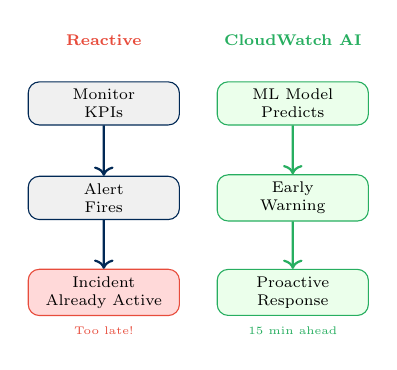
\begin{tikzpicture}[scale=0.8, transform shape,
  box/.style={rectangle, rounded corners, draw=UNBBlue, fill=UNBLightGray, minimum width=2.4cm, minimum height=0.65cm, font=\scriptsize, align=center},
  goodbox/.style={rectangle, rounded corners, draw=UNBGreen, fill=green!8, minimum width=2.4cm, minimum height=0.65cm, font=\scriptsize, align=center},
  arrow/.style={->, thick, UNBBlue},
  garrow/.style={->, thick, UNBGreen}
]
% Reactive (left)
\node[font=\scriptsize\bfseries, UNBRed] at (-1.5,4) {Reactive};
\node[box] (monitor) at (-1.5,3) {Monitor\\KPIs};
\node[box] (alert) at (-1.5,1.5) {Alert\\Fires};
\node[box, fill=red!15, draw=UNBRed] (incident) at (-1.5,0) {Incident\\Already Active};

\draw[arrow] (monitor) -- (alert);
\draw[arrow] (alert) -- (incident);

% Predictive (right)
\node[font=\scriptsize\bfseries, UNBGreen] at (1.5,4) {CloudWatch AI};
\node[goodbox] (ml) at (1.5,3) {ML Model\\Predicts};
\node[goodbox] (early) at (1.5,1.5) {Early\\Warning};
\node[goodbox] (prevent) at (1.5,0) {Proactive\\Response};

\draw[garrow] (ml) -- (early);
\draw[garrow] (early) -- (prevent);

\node[font=\tiny, UNBRed] at (-1.5,-0.6) {Too late!};
\node[font=\tiny, UNBGreen] at (1.5,-0.6) {15 min ahead};
\end{tikzpicture}
\end{column}
\end{columns}
\end{frame}

% ===== SLIDE 3: KEY FEATURES =====
\begin{frame}{Key Features}
\framesubtitle{What Makes CloudWatch AI Unique}

\begin{columns}[T]
\begin{column}{0.48\textwidth}
\begin{block}{Predictive Intelligence}
\begin{itemize}
    \item 3 ML models for 5, 10, 15-min horizons
    \item 8 engineered features (KPI + Log signals)
    \item Calibrated thresholds per service
    \item Lead time: $\sim$36 minutes average
\end{itemize}
\end{block}

\vspace{0.3em}
\begin{block}{Real-Time Simulation}
\begin{itemize}
    \item 5 monitored cloud services
    \item Realistic incident scenarios
    \item Live data generation every 1 minute
    \item Event-driven pipeline via DynamoDB Streams
\end{itemize}
\end{block}
\end{column}

\begin{column}{0.48\textwidth}
\begin{block}{Interactive Dashboard}
\begin{itemize}
    \item 4 pages: Live Controls, KPI Timeline, Alerts, Analytics
    \item Dark/Light theme with persistent preference
    \item Real-time chart updates via polling
    \item Alert management with incident grouping
\end{itemize}
\end{block}

\vspace{0.3em}
\begin{block}{Enterprise Security}
\begin{itemize}
    \item AWS Cognito authentication (SRP protocol)
    \item JWT authorizer on all 16 API routes
    \item AES-256 encryption at rest
    \item TLS 1.2+ encryption in transit
\end{itemize}
\end{block}
\end{column}
\end{columns}
\end{frame}

% ===== SLIDE 4: SYSTEM ARCHITECTURE =====
\begin{frame}{System Architecture}
\framesubtitle{Serverless, Event-Driven Architecture on AWS}

\centering
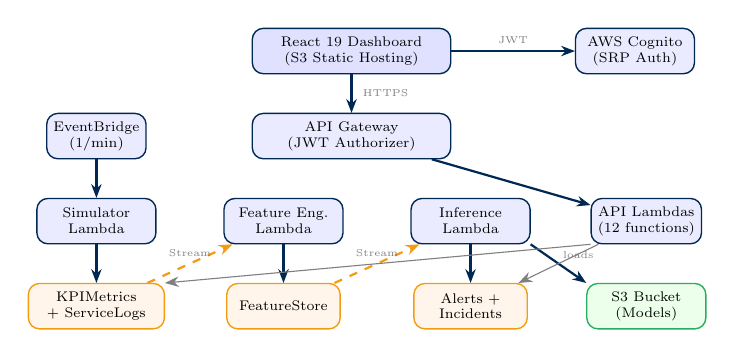
\begin{tikzpicture}[
  scale=0.72, transform shape,
  box/.style={rectangle, rounded corners=4pt, draw=UNBBlue, fill=UNBLightGray, minimum width=2.1cm, minimum height=0.8cm, font=\scriptsize, align=center, line width=0.5pt},
  awsbox/.style={rectangle, rounded corners=4pt, draw=UNBBlue, fill=blue!8, minimum width=2.1cm, minimum height=0.8cm, font=\scriptsize, align=center, line width=0.5pt},
  dbbox/.style={rectangle, rounded corners=4pt, draw=UNBOrange, fill=orange!8, minimum width=2.1cm, minimum height=0.8cm, font=\scriptsize, align=center, line width=0.5pt},
  s3box/.style={rectangle, rounded corners=4pt, draw=UNBGreen, fill=green!8, minimum width=2.1cm, minimum height=0.8cm, font=\scriptsize, align=center, line width=0.5pt},
  arrow/.style={-{Stealth[length=5pt]}, thick, UNBBlue},
  stream/.style={-{Stealth[length=5pt]}, thick, UNBOrange, dashed},
  label/.style={font=\tiny, UNBGray}
]

% Row 1: User + Frontend
\node[box, minimum width=3.5cm, fill=blue!12] (browser) at (0,4.5) {React 19 Dashboard\\(S3 Static Hosting)};
\node[awsbox] (cognito) at (5,4.5) {AWS Cognito\\(SRP Auth)};

% Row 2: API Gateway
\node[awsbox, minimum width=3.5cm] (apigw) at (0,3) {API Gateway\\(JWT Authorizer)};

% Row 3: Lambda functions
\node[awsbox] (simulator) at (-4.5,1.5) {Simulator\\Lambda};
\node[awsbox] (feateng) at (-1.2,1.5) {Feature Eng.\\Lambda};
\node[awsbox] (inference) at (2.1,1.5) {Inference\\Lambda};
\node[awsbox, minimum width=1.8cm] (apilambda) at (5.2,1.5) {API Lambdas\\(12 functions)};

% Row 4: Data stores
\node[dbbox, minimum width=2.4cm] (kpi) at (-4.5,0) {KPIMetrics\\+ ServiceLogs};
\node[dbbox, minimum width=2.0cm] (features) at (-1.2,0) {FeatureStore};
\node[dbbox, minimum width=2.0cm] (alerts) at (2.1,0) {Alerts +\\Incidents};
\node[s3box] (s3) at (5.2,0) {S3 Bucket\\(Models)};

% EventBridge
\node[awsbox, minimum width=1.6cm] (eventbridge) at (-4.5,3) {EventBridge\\(1/min)};

% Arrows
\draw[arrow] (browser) -- node[label, right, xshift=2pt] {HTTPS} (apigw);
\draw[arrow] (browser) -- node[label, above] {JWT} (cognito);
\draw[arrow] (apigw) -- (apilambda);
\draw[arrow] (eventbridge) -- (simulator);

% Data flow
\draw[arrow] (simulator) -- (kpi);
\draw[stream] (kpi) -- node[label, above] {Stream} (feateng);
\draw[arrow] (feateng) -- (features);
\draw[stream] (features) -- node[label, above] {Stream} (inference);
\draw[arrow] (inference) -- (alerts);
\draw[arrow] (inference.south east) -- (s3.north west);
\node[label] at (4.0,0.9) {loads};

% API reads
\draw[arrow, gray, thin] (apilambda) -- (alerts);
\draw[arrow, gray, thin] (apilambda.south west) -- (kpi.north east);

\end{tikzpicture}

\vspace{0.3em}
{\small
\textbf{Key:} Solid arrows = direct calls. Dashed orange = DynamoDB Stream triggers (automatic, event-driven).\\
12 Lambda functions total, all serverless. Entire platform runs within AWS Free Tier.
}
\end{frame}

% ===== SLIDE 5: TECH STACK =====
\begin{frame}{Technology Stack}
\framesubtitle{AWS Services and Open-Source Tools}

\begin{columns}[T]
\begin{column}{0.48\textwidth}
\begin{block}{Frontend}
{\small
\begin{tabular}{ll}
\toprule
\textbf{Technology} & \textbf{Purpose} \\
\midrule
React 19 + TypeScript & UI framework \\
Vite 7 & Build tool \\
Tailwind CSS 4 & Styling \\
Recharts 3.8 & Charts \\
Cognito SDK & Authentication \\
React Router 7 & Navigation \\
\bottomrule
\end{tabular}
}
\end{block}
\end{column}

\begin{column}{0.48\textwidth}
\begin{block}{Backend \& Infrastructure}
{\small
\begin{tabular}{ll}
\toprule
\textbf{Service} & \textbf{Purpose} \\
\midrule
AWS Lambda & Compute (Python) \\
DynamoDB & Database (6 tables) \\
API Gateway & HTTP API (16 routes) \\
S3 & Static hosting + models \\
EventBridge & Scheduler (1/min) \\
Cognito & Authentication \\
\bottomrule
\end{tabular}
}
\end{block}
\end{column}
\end{columns}

\vspace{0.4em}
\begin{block}{ML Pipeline}
{\small
\begin{tabular}{lll}
\toprule
\textbf{Component} & \textbf{Technology} & \textbf{Details} \\
\midrule
Model & scikit-learn GBC & 100 trees, depth 3, LR 0.1 \\
Training Data & AIOps KPI Dataset & 2.4M timesteps, 26 services \\
Deployment & Docker on Lambda & Container image from ECR \\
\bottomrule
\end{tabular}
}
\end{block}
\end{frame}

% ===== SLIDE 6: DATA MODEL =====
\begin{frame}{Data Model}
\framesubtitle{DynamoDB -- Flexible Schema for Heterogeneous Cloud Services}

\begin{columns}[T]
\begin{column}{0.52\textwidth}
\begin{block}{6 DynamoDB Tables}
{\footnotesize
\begin{tabular}{lp{1.4cm}p{1.2cm}l}
\toprule
\textbf{Table} & \textbf{PK} & \textbf{SK} & \textbf{Purpose} \\
\midrule
KPIMetrics & service\_id & timestamp & Raw metrics \\
ServiceLogs & service\_id & timestamp & Event logs \\
FeatureStore & service\_id & timestamp & 8 features \\
Alerts & alert\_id & -- & Predictions \\
Incidents & incident\_id & -- & Grouped alerts \\
SimConfig & config\_key & -- & Sim state \\
\bottomrule
\end{tabular}
}
\end{block}

\vspace{0.3em}
\begin{alertblock}{Why DynamoDB?}
{\small Each service type produces \textbf{different JSON fields}. DynamoDB's flexible schema stores heterogeneous documents in one table --- no nullable columns needed.}
\end{alertblock}
\end{column}

\begin{column}{0.44\textwidth}
\begin{block}{Variable Schema per Service}
{\scriptsize
\textbf{Web API:} response\_time\_ms, requests/sec, error\_rate, http\_5xx\_count\\[3pt]
\textbf{DB Pool:} active\_connections, query\_duration, deadlock\_count\\[3pt]
\textbf{Message Queue:} queue\_depth, consumer\_lag, dead\_letter\_size\\[3pt]
\textbf{Auth Service:} login\_success\_rate, auth\_latency, mfa\_rate\\[3pt]
\textbf{ML Pipeline:} inference\_latency, accuracy, drift\_score
}
\end{block}

\vspace{0.3em}
\begin{block}{NoSQL Design Choices}
{\small
\begin{itemize}
    \item \textbf{Partition key} = service\_id (query by service)
    \item \textbf{Sort key} = timestamp (time-range queries)
    \item \textbf{TTL} on all data tables (24h auto-cleanup)
    \item \textbf{DynamoDB Streams} trigger pipeline Lambdas
\end{itemize}
}
\end{block}
\end{column}
\end{columns}
\end{frame}

% ===== SLIDE 7: DATA FLOW PIPELINE =====
\begin{frame}{Data Flow Pipeline}
\framesubtitle{Event-Driven, Fully Automatic Processing}

\centering
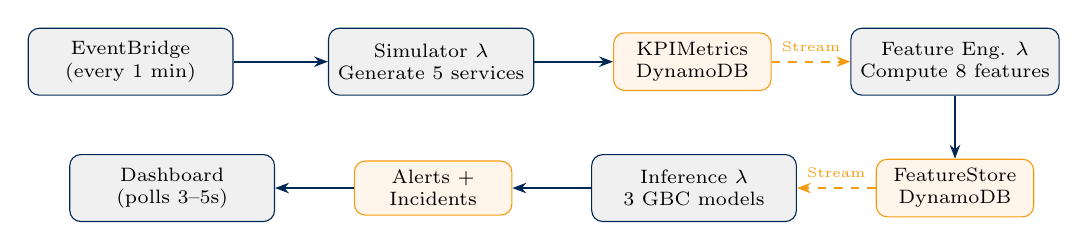
\begin{tikzpicture}[node distance=1.4cm, every node/.style={font=\small},
  box/.style={rectangle, rounded corners, draw=UNBBlue, fill=UNBLightGray, minimum width=2.6cm, minimum height=0.85cm, align=center, font=\scriptsize},
  dbbox/.style={rectangle, rounded corners, draw=UNBOrange, fill=orange!8, minimum width=2.0cm, minimum height=0.65cm, align=center, font=\scriptsize},
  arrow/.style={-{Stealth[length=5pt]}, thick, UNBBlue},
  stream/.style={-{Stealth[length=5pt]}, thick, UNBOrange, dashed}
]

% Pipeline steps
\node[box] (eb) at (0,0) {EventBridge\\(every 1 min)};
\node[box, right=1.2cm of eb] (sim) {Simulator $\lambda$\\Generate 5 services};
\node[dbbox, right=1.0cm of sim] (kpi) {KPIMetrics\\DynamoDB};
\node[box, right=1.0cm of kpi] (feat) {Feature Eng. $\lambda$\\Compute 8 features};
\node[dbbox, below=0.8cm of feat] (fs) {FeatureStore\\DynamoDB};
\node[box, left=1.0cm of fs] (inf) {Inference $\lambda$\\3 GBC models};
\node[dbbox, left=1.0cm of inf] (alrt) {Alerts +\\Incidents};
\node[box, left=1.0cm of alrt] (dash) {Dashboard\\(polls 3--5s)};

% Arrows
\draw[arrow] (eb) -- (sim);
\draw[arrow] (sim) -- (kpi);
\draw[stream] (kpi) -- node[above, font=\tiny, UNBOrange] {Stream} (feat);
\draw[arrow] (feat) -- (fs);
\draw[stream] (fs) -- node[above, font=\tiny, UNBOrange] {Stream} (inf);
\draw[arrow] (inf) -- (alrt);
\draw[arrow] (alrt) -- (dash);

\end{tikzpicture}

\vspace{0.6em}
\begin{columns}[T]
\begin{column}{0.48\textwidth}
\begin{block}{Simulation Scenarios}
{\small
\begin{itemize}
    \item \textbf{Web API Degradation} -- response times spike, cascade to DB
    \item \textbf{DB Cascade Failure} -- deadlocks trigger multi-service impact
    \item \textbf{Baseline} -- normal operations, no incident
\end{itemize}
}
\end{block}
\end{column}
\begin{column}{0.48\textwidth}
\begin{block}{Scenario Timeline (15 min)}
{\small
\begin{tabular}{ll}
Min 0--5 & All services normal \\
Min 5--7 & Response times creep up \\
Min 7--8 & \textbf{Model fires alert} \\
Min 9--12 & Full incident develops \\
Min 12--15 & Recovery phase \\
\end{tabular}
}
\end{block}
\end{column}
\end{columns}
\end{frame}

% ===== SLIDE 8: ML MODEL =====
\begin{frame}{ML Model}
\framesubtitle{Gradient Boosting Classifier with KPI + Log-Proxy Features}

\begin{columns}[T]
\begin{column}{0.45\textwidth}
\begin{block}{Model Configuration}
{\small
\begin{tabular}{ll}
\toprule
\textbf{Parameter} & \textbf{Value} \\
\midrule
Algorithm & GBC (scikit-learn) \\
Trees & 100 \\
Max Depth & 3 \\
Learning Rate & 0.1 \\
Horizons & 5, 10, 15 min \\
Training Data & 2.4M timesteps \\
\bottomrule
\end{tabular}
}
\end{block}

\vspace{0.3em}
\begin{alertblock}{Alert Calibration}
{\small Thresholds tuned per service so that at most \textbf{1 false alarm per 24 hours}. Frozen after training for consistent deployment.}
\end{alertblock}
\end{column}

\begin{column}{0.52\textwidth}
\begin{block}{8 Engineered Features}
{\small
\begin{tabular}{lll}
\toprule
\textbf{Feature} & \textbf{Type} & \textbf{Import.} \\
\midrule
roll\_mean & KPI & 31.1\% \\
error\_rate & \textcolor{UNBRed}{Log} & \textcolor{UNBRed}{26.6\%} \\
roll\_max & KPI & 19.8\% \\
roll\_std & KPI & 12.9\% \\
severity\_change & \textcolor{UNBRed}{Log} & \textcolor{UNBRed}{4.6\%} \\
first\_diff & KPI & 3.5\% \\
roll\_slope & KPI & 1.0\% \\
warn\_rate & \textcolor{UNBRed}{Log} & \textcolor{UNBRed}{0.4\%} \\
\bottomrule
\end{tabular}
}
\end{block}

\vspace{0.2em}
{\small \textbf{Key insight:} Log-proxy features (red) contribute \textbf{31.6\%} of total importance --- multi-signal fusion is essential.}
\end{column}
\end{columns}
\end{frame}

% ===== SLIDE 9: MODEL PERFORMANCE =====
\begin{frame}{Model Performance}
\framesubtitle{Best Result: GBC with KPI + Log Features at H=15}

\begin{columns}
\begin{column}{0.45\textwidth}
\begin{block}{Performance Metrics}
{\small
\begin{tabular}{ll}
\toprule
\textbf{Metric} & \textbf{Value} \\
\midrule
Precision & \textbf{0.91} \\
Mean Lead Time & \textbf{$\sim$36 min} \\
False Alarm Rate & $\leq$ 1/day/service \\
Detection Rate & 8.7\% \\
\bottomrule
\end{tabular}
}
\end{block}

\vspace{0.4em}
\begin{block}{KPI-Only vs KPI+Logs}
{\small
\begin{tabular}{lcc}
\toprule
\textbf{Model} & \textbf{Prec.} & \textbf{Rec.} \\
\midrule
GBC KPI+Logs & \textbf{0.91} & \textbf{0.43} \\
GBC KPI Only & 0.63 & 0.16 \\
Static Baseline & 0.63 & 0.47 \\
Moving Avg. & 0.42 & 0.02 \\
\bottomrule
\end{tabular}
}
\end{block}
\end{column}

\begin{column}{0.5\textwidth}
\centering
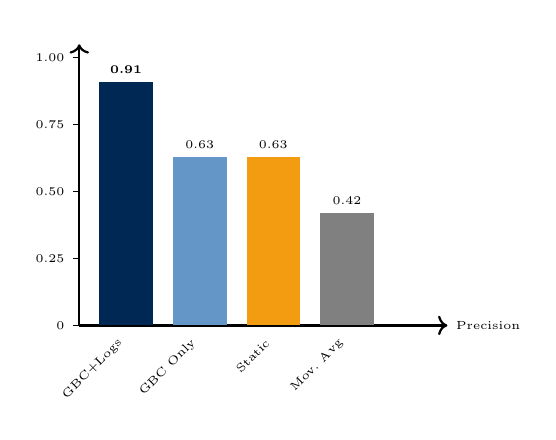
\begin{tikzpicture}[scale=0.85, transform shape]
% Precision bar chart (simplified)
\draw[thick, ->] (0,0) -- (5.5,0) node[right, font=\tiny] {Precision};
\draw[thick, ->] (0,0) -- (0,4.2) node[above, font=\tiny] {};

% Bars
\fill[UNBBlue] (0.3,0) rectangle (1.1,3.64); % GBC KPI+Logs 0.91
\fill[UNBLightBlue] (1.4,0) rectangle (2.2,2.52); % GBC KPI Only 0.63
\fill[UNBOrange] (2.5,0) rectangle (3.3,2.52); % Static 0.63
\fill[UNBGray] (3.6,0) rectangle (4.4,1.68); % MA 0.42

% Labels
\node[font=\tiny, rotate=45, anchor=east] at (0.7,-0.15) {GBC+Logs};
\node[font=\tiny, rotate=45, anchor=east] at (1.8,-0.15) {GBC Only};
\node[font=\tiny, rotate=45, anchor=east] at (2.9,-0.15) {Static};
\node[font=\tiny, rotate=45, anchor=east] at (4.0,-0.15) {Mov.~Avg};

% Value labels
\node[font=\tiny\bfseries, above] at (0.7,3.64) {0.91};
\node[font=\tiny, above] at (1.8,2.52) {0.63};
\node[font=\tiny, above] at (2.9,2.52) {0.63};
\node[font=\tiny, above] at (4.0,1.68) {0.42};

% Y-axis ticks
\foreach \y/\l in {0/0, 1/0.25, 2/0.50, 3/0.75, 4/1.00} {
    \draw (0,\y) -- (-0.1,\y) node[left, font=\tiny] {\l};
}
\end{tikzpicture}

\vspace{0.3em}
\begin{alertblock}{Key Finding}
{\small The main operational benefit: \textbf{more trustworthy alerts with less alert fatigue}, not just earlier detection.}
\end{alertblock}
\end{column}
\end{columns}
\end{frame}

% ===== SLIDE 10: IMPLEMENTATION -- DASHBOARD =====
\begin{frame}{Implementation: Dashboard}
\framesubtitle{React 19 Single-Page Application with 4 Interactive Pages}

\begin{columns}[T]
\begin{column}{0.48\textwidth}

\begin{block}{Page 1: Live Controls}
{\small
\begin{itemize}
    \item Start/Stop simulation scenarios
    \item Scenario selector dropdown
    \item 5 Service Health Cards with live status
    \item Summary cards: phase, tick, predictions
\end{itemize}
}
\end{block}

\vspace{0.2em}
\begin{block}{Page 2: KPI Timeline}
{\small
\begin{itemize}
    \item Real-time scrolling line charts (Recharts)
    \item Service tabs + ``All Services'' overlay
    \item Prediction score chart with threshold line
    \item Horizon toggle: 5m / 10m / 15m
\end{itemize}
}
\end{block}
\end{column}

\begin{column}{0.48\textwidth}
\begin{block}{Page 3: Alerts \& Incidents}
{\small
\begin{itemize}
    \item Active alerts with severity badges (Critical/Warning/Info)
    \item Acknowledge and dismiss actions
    \item Incident groups with colored phase timeline
    \item Collapsible alert history section
\end{itemize}
}
\end{block}

\vspace{0.2em}
\begin{block}{Page 4: Analytics}
{\small
\begin{itemize}
    \item Summary stats: precision, lead time, FAR
    \item Precision vs Detection Rate scatter chart
    \item Lead Time Distribution bar chart
    \item Feature Importance chart (KPI vs Log)
\end{itemize}
}
\end{block}
\end{column}
\end{columns}

\vspace{0.3em}
\centering
{\small \textit{[Screenshot placeholders: insert dashboard screenshots on next slide]}}
\end{frame}

% ===== SLIDE 11: IMPLEMENTATION -- DASHBOARD SCREENSHOTS =====
\begin{frame}{Dashboard Screenshots}
\framesubtitle{Live Controls \& KPI Timeline}

\begin{columns}
\begin{column}{0.48\textwidth}
\centering
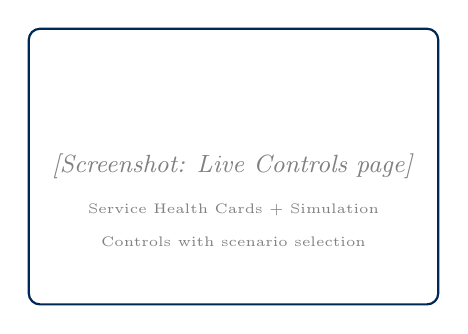
\begin{tikzpicture}
\draw[UNBBlue, thick, rounded corners=4pt] (0,0) rectangle (5.2,3.5);
\node[font=\small, UNBGray] at (2.6,1.75) {\textit{[Screenshot: Live Controls page]}};
\node[font=\tiny, UNBGray] at (2.6,1.2) {Service Health Cards + Simulation};
\node[font=\tiny, UNBGray] at (2.6,0.8) {Controls with scenario selection};
\end{tikzpicture}
\end{column}
\begin{column}{0.48\textwidth}
\centering
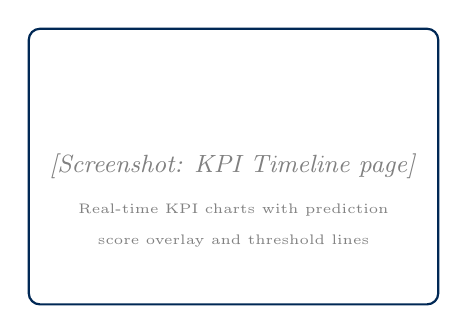
\begin{tikzpicture}
\draw[UNBBlue, thick, rounded corners=4pt] (0,0) rectangle (5.2,3.5);
\node[font=\small, UNBGray] at (2.6,1.75) {\textit{[Screenshot: KPI Timeline page]}};
\node[font=\tiny, UNBGray] at (2.6,1.2) {Real-time KPI charts with prediction};
\node[font=\tiny, UNBGray] at (2.6,0.8) {score overlay and threshold lines};
\end{tikzpicture}
\end{column}
\end{columns}

\vspace{0.5em}
\begin{columns}
\begin{column}{0.48\textwidth}
\centering
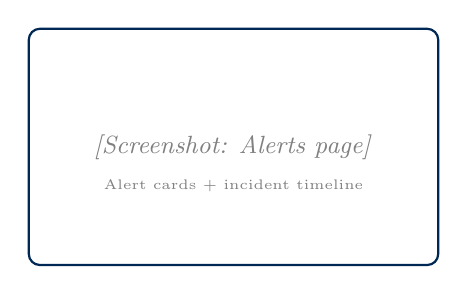
\begin{tikzpicture}
\draw[UNBBlue, thick, rounded corners=4pt] (0,0) rectangle (5.2,3.0);
\node[font=\small, UNBGray] at (2.6,1.5) {\textit{[Screenshot: Alerts page]}};
\node[font=\tiny, UNBGray] at (2.6,1.0) {Alert cards + incident timeline};
\end{tikzpicture}
\end{column}
\begin{column}{0.48\textwidth}
\centering
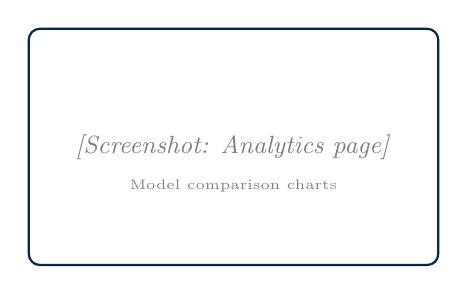
\begin{tikzpicture}
\draw[UNBBlue, thick, rounded corners=4pt] (0,0) rectangle (5.2,3.0);
\node[font=\small, UNBGray] at (2.6,1.5) {\textit{[Screenshot: Analytics page]}};
\node[font=\tiny, UNBGray] at (2.6,1.0) {Model comparison charts};
\end{tikzpicture}
\end{column}
\end{columns}
\end{frame}

% ===== SLIDE 12: IMPLEMENTATION -- BACKEND =====
\begin{frame}{Implementation: Backend}
\framesubtitle{12 Lambda Functions with Event-Driven Processing}

\begin{columns}[T]
\begin{column}{0.48\textwidth}
\begin{block}{Lambda Functions (from AWS)}
{\footnotesize
\begin{tabular}{ll}
\toprule
\textbf{Function} & \textbf{Trigger} \\
\midrule
simulator\_lambda & EventBridge \\
feature\_engineering & DynamoDB Stream \\
inference\_lambda & DynamoDB Stream \\
\midrule
services\_lambda & API Gateway \\
kpi\_lambda & API Gateway \\
alerts\_lambda & API Gateway \\
incidents\_lambda & API Gateway \\
analytics\_lambda & API Gateway \\
threshold\_lambda & API Gateway \\
control\_simulation & API Gateway \\
get\_metrics\_lambda & API Gateway \\
get\_logs\_lambda & API Gateway \\
\bottomrule
\end{tabular}
}
\end{block}
\end{column}

\begin{column}{0.48\textwidth}
\begin{block}{Inference Lambda Details}
{\small
\begin{itemize}
    \item Deployed as \textbf{Docker container} on Lambda
    \item Loads 3 trained GBC models from S3
    \item \textbf{Model caching} avoids re-download
    \item Processes DynamoDB Stream events
    \item Creates alerts when score $>$ threshold
    \item Groups $\geq$2 related alerts into incidents
\end{itemize}
}
\end{block}

\vspace{0.3em}
\begin{block}{API Gateway Configuration}
{\small
\begin{itemize}
    \item HTTP API with \textbf{16 routes}
    \item All routes protected by \textbf{JWT Authorizer}
    \item CORS configured for frontend origin
    \item Rate limiting: 10K req/s burst
\end{itemize}
}
\end{block}
\end{column}
\end{columns}
\end{frame}

% ===== SLIDE 13: SECURITY =====
\begin{frame}{Security Architecture}
\framesubtitle{Authentication, Authorization, and Encryption}

\begin{columns}[T]
\begin{column}{0.48\textwidth}
\begin{block}{Authentication (AWS Cognito)}
{\small
\begin{itemize}
    \item SRP protocol (password never sent in plaintext)
    \item Email verification required
    \item Password policy: min 8 chars, upper + lower + number
    \item JWT tokens: ID (1h), Refresh (30d)
\end{itemize}
}
\end{block}

\vspace{0.3em}
\begin{block}{Encryption}
{\small
\begin{tabular}{ll}
\toprule
\textbf{Scope} & \textbf{Method} \\
\midrule
DynamoDB at rest & AES-256 (AWS keys) \\
S3 at rest & AES-256 (SSE-S3) \\
API calls in transit & TLS 1.2+ \\
Auth in transit & TLS 1.2+ \\
AWS internal & TLS 1.2+ \\
\bottomrule
\end{tabular}
}
\end{block}
\end{column}

\begin{column}{0.48\textwidth}
\begin{block}{Authorization}
{\small
\begin{itemize}
    \item API Gateway JWT Authorizer on \textbf{all 16 routes}
    \item Frontend ProtectedRoute component
    \item 401 response $\rightarrow$ auto-redirect to /login
\end{itemize}
}
\end{block}

\vspace{0.3em}
\begin{block}{Access Controls}
{\small
\begin{itemize}
    \item Least-privilege IAM roles for Lambda
    \item No direct public access to DynamoDB
    \item S3: public read for frontend only
    \item No hardcoded secrets in source code
\end{itemize}
}
\end{block}

\vspace{0.3em}
\begin{alertblock}{Verification}
{\footnotesize
\texttt{curl .../services} $\rightarrow$ \texttt{\{"message":"Unauthorized"\}}\\
HTTP 401 without valid JWT token.
}
\end{alertblock}
\end{column}
\end{columns}
\end{frame}

% ===== SLIDE 14: OWASP + TESTING =====
\begin{frame}{Security Audit \& Testing}
\framesubtitle{OWASP Top 10 Assessment + Integration Test Results}

\begin{columns}[T]
\begin{column}{0.48\textwidth}
\begin{block}{OWASP Top 10 Results}
{\scriptsize
\begin{tabular}{lll}
\toprule
\textbf{\#} & \textbf{Vulnerability} & \textbf{Status} \\
\midrule
A01 & Broken Access Control & \textcolor{UNBGreen}{\textbf{Pass}} \\
A02 & Cryptographic Failures & \textcolor{UNBGreen}{\textbf{Pass}} \\
A03 & Injection & \textcolor{UNBGreen}{\textbf{Pass}} \\
A04 & Insecure Design & \textcolor{UNBGreen}{\textbf{Pass}} \\
A05 & Security Misconfig. & \textcolor{UNBGreen}{\textbf{Pass}} \\
A06 & Vulnerable Components & \textcolor{UNBGreen}{\textbf{Pass}} \\
A07 & Auth Failures & \textcolor{UNBGreen}{\textbf{Pass}} \\
A08 & Data Integrity & \textcolor{UNBGreen}{\textbf{Pass}} \\
A09 & Security Logging & \textcolor{UNBGreen}{\textbf{Pass}} \\
A10 & SSRF & N/A \\
\bottomrule
\end{tabular}
}
\end{block}
\vspace{0.2em}
{\small \textbf{Score: 9/10 passed}, 1 N/A. Overall risk: \textcolor{UNBGreen}{\textbf{Low}}.}
\end{column}

\begin{column}{0.48\textwidth}
\begin{block}{Integration Testing Summary}
{\small
\begin{tabular}{lc}
\toprule
\textbf{Category} & \textbf{Tests} \\
\midrule
Authentication (CLI) & 5 passed \\
API Endpoints & 16 tested \\
Simulation Lifecycle & Verified \\
Database Integrity & Verified \\
Production Deployment & Verified \\
\midrule
Authentication (Browser) & 4 planned \\
Frontend Integration & 17 planned \\
Cross-Cutting (Theme, etc.) & 7 planned \\
\midrule
\textbf{Total} & \textbf{50+ cases} \\
\bottomrule
\end{tabular}
}
\end{block}

\vspace{0.2em}
\begin{alertblock}{Additional Checks}
{\footnotesize CORS, Rate Limiting, Input Validation, Error Handling, Secrets Management, DynamoDB TTL --- all passed.}
\end{alertblock}
\end{column}
\end{columns}
\end{frame}

% ===== SLIDE 15: CHALLENGES AND SOLUTIONS =====
\begin{frame}{Challenges and Solutions}
\framesubtitle{Key Obstacles Encountered During Implementation}

\begin{columns}[T]
\begin{column}{0.48\textwidth}
\begin{block}{Challenge 1: Low Recall vs High Precision}
{\small
\textbf{Problem:} Detection rate was only 8.7\%\\
\textbf{Solution:} Prioritized precision (0.91) for operator trust. High recall with many false alarms is worse than selective, trustworthy alerts.\\
\textbf{Lesson:} In AIOps, precision $>$ recall for operational adoption.
}
\end{block}

\vspace{0.3em}
\begin{block}{Challenge 2: Cold Start Latency}
{\small
\textbf{Problem:} Lambda cold starts delayed inference when loading scikit-learn models.\\
\textbf{Solution:} Docker container deployment + model caching in Lambda global scope. Models load once and persist across invocations.
}
\end{block}
\end{column}

\begin{column}{0.48\textwidth}
\begin{block}{Challenge 3: Heterogeneous Data Schema}
{\small
\textbf{Problem:} 5 services produce completely different JSON structures.\\
\textbf{Solution:} Used DynamoDB's flexible schema --- each service stores its own document shape. Feature Engineering extracts one primary metric per service for the model.
}
\end{block}

\vspace{0.3em}
\begin{block}{Challenge 4: Real-Time Pipeline Orchestration}
{\small
\textbf{Problem:} Needed automatic, event-driven data flow without polling.\\
\textbf{Solution:} DynamoDB Streams trigger Lambdas automatically: KPIMetrics $\rightarrow$ Feature Eng. $\rightarrow$ Inference. Zero orchestration code needed.
}
\end{block}
\end{column}
\end{columns}
\end{frame}

% ===== SLIDE 16: LIVE DEMO FLOW =====
\begin{frame}{Live Demo}
\framesubtitle{Watch the Model Detect an Incident in Real Time}

\centering
\begin{tikzpicture}[
  node distance=0.6cm,
  step/.style={rectangle, rounded corners=4pt, draw=UNBBlue, fill=UNBLightGray, minimum width=11cm, minimum height=0.55cm, font=\small, align=left},
  highlight/.style={rectangle, rounded corners=4pt, draw=UNBGreen, fill=green!10, minimum width=11cm, minimum height=0.55cm, font=\small\bfseries, align=left},
  num/.style={circle, draw=UNBBlue, fill=UNBBlue, text=white, font=\tiny\bfseries, minimum size=0.4cm, inner sep=0pt}
]

\node[step] (s1) {Open dashboard \& select ``Web API Degradation'' scenario};
\node[step, below=of s1] (s2) {Click Start Simulation --- EventBridge begins generating data};
\node[step, below=of s2] (s3) {Watch KPI Timeline --- all services show normal behavior (min 0--5)};
\node[step, below=of s3] (s4) {Web API response times start creeping up (min 5--7)};
\node[highlight, below=of s4] (s5) {Prediction score rises --- model fires alert \textbf{before} full incident (min 7--8)};
\node[step, below=of s5] (s6) {Full incident develops across Web API + DB Pool (min 9--12)};
\node[step, below=of s6] (s7) {Recovery phase --- metrics trend back to normal (min 12--15)};
\node[step, below=of s7] (s8) {Switch to Analytics page --- view precision, lead time, feature importance};

% Numbers
\node[num] at ([xshift=-5.9cm]s1.west) {1};
\node[num] at ([xshift=-5.9cm]s2.west) {2};
\node[num] at ([xshift=-5.9cm]s3.west) {3};
\node[num] at ([xshift=-5.9cm]s4.west) {4};
\node[num] at ([xshift=-5.9cm]s5.west) {5};
\node[num] at ([xshift=-5.9cm]s6.west) {6};
\node[num] at ([xshift=-5.9cm]s7.west) {7};
\node[num] at ([xshift=-5.9cm]s8.west) {8};

\end{tikzpicture}

\vspace{0.3em}
{\small Total demo time: $\sim$10--15 minutes. The model provides early warning 2+ minutes before the incident fully develops.}
\end{frame}

% ===== SLIDE 17: CONCLUSION =====
\begin{frame}{Conclusion}
\framesubtitle{Summary of Achievements}

\begin{columns}
\begin{column}{0.58\textwidth}
\begin{block}{What We Built}
\begin{enumerate}
    \item A \textbf{fully serverless} AIOps platform on AWS
    \item \textbf{ML-powered} incident prediction with 0.91 precision
    \item \textbf{Event-driven} pipeline: data $\rightarrow$ features $\rightarrow$ alerts (automatic)
    \item \textbf{Interactive dashboard} with real-time visualization
    \item \textbf{Comprehensive security}: Cognito auth, JWT, AES-256, OWASP audit
\end{enumerate}
\end{block}

\vspace{0.3em}
\begin{block}{Key Numbers}
{\small
\begin{tabular}{ll}
12 Lambda Functions & 6 DynamoDB Tables \\
16 API Routes (JWT) & 5 Monitored Services \\
3 ML Models & 50+ Test Cases \\
8 Engineered Features & 9/10 OWASP Passed \\
\end{tabular}
}
\end{block}
\end{column}

\begin{column}{0.38\textwidth}
\begin{alertblock}{Core Achievement}
{\small Predictive models don't just detect earlier --- they produce \textbf{more trustworthy alerts} with \textbf{fewer false alarms}, leading to higher operator trust.}
\end{alertblock}

\vspace{0.3em}
\begin{block}{Practical Impact}
{\small
Fewer false alarms\\
$\downarrow$\\
Higher on-call trust\\
$\downarrow$\\
Faster incident response\\
$\downarrow$\\
\textbf{Better cloud reliability}
}
\end{block}
\end{column}
\end{columns}
\end{frame}

% ===== SLIDE 18: FUTURE WORK =====
\begin{frame}{Future Work}
\framesubtitle{Potential Improvements and Extensions}

\begin{columns}[T]
\begin{column}{0.48\textwidth}
\begin{block}{Technical Extensions}
\begin{itemize}
    \item Replace synthetic log-proxies with \textbf{real system logs}
    \item Add \textbf{cross-service correlation} for cascading failure detection
    \item Test deeper models: \textbf{LSTM}, \textbf{Transformer}
    \item \textbf{Hyperparameter tuning} for improved recall
    \item Add \textbf{CloudFront CDN} for HTTPS frontend hosting
\end{itemize}
\end{block}
\end{column}

\begin{column}{0.48\textwidth}
\begin{block}{Operational Improvements}
\begin{itemize}
    \item \textbf{Online model updating} for concept drift
    \item Real production traffic integration
    \item \textbf{Multi-metric models} per service
    \item Automated \textbf{CI/CD pipeline} for model retraining
    \item Role-based access control (admin vs viewer)
\end{itemize}
\end{block}
\end{column}
\end{columns}

\vspace{0.5em}
\begin{block}{Known Limitations (Transparency)}
{\small
\begin{tabular}{ll}
\textbf{Limitation} & \textbf{Rationale} \\
\midrule
Low recall (8.7\%) & Precision prioritized for operator trust \\
Synthetic data & Controlled scenarios for consistent demos \\
One metric per service & Simplicity; multi-metric is a future extension \\
\end{tabular}
}
\end{block}
\end{frame}

% ===== SLIDE 19: THANK YOU =====
\begin{frame}

\begin{center}
\setbeamercolor{block title}{bg=UNBBlue,fg=white}
\setbeamercolor{block body}{bg=UNBBlue,fg=white}
\begin{block}{}
\centering
\textbf{Thank you for your attention!}
\end{block}

\vspace{0.5em}
{\normalsize Questions?}

\vspace{1em}
{\small
\textbf{Team:} Akinbobola Akin $\cdot$ Alfarizy Alfarizy $\cdot$ Ishimwe Pacis Hanyurwimfura\\[0.5em]
\textbf{Live Dashboard:}\\
\texttt{cloud-project-dashboard1.s3-website.ca-central-1.amazonaws.com}\\[0.5em]
\textbf{API Endpoint:}\\
\texttt{p9fpx4nhh6.execute-api.ca-central-1.amazonaws.com}
}
\end{center}
\end{frame}

% ================================================================
% BACKUP SLIDES (for Q\&A)
% ================================================================

% ===== BACKUP 1: AWS RESOURCES =====
\begin{frame}{Backup: AWS Resources (Live)}
\framesubtitle{Verified via AWS CLI on March 22, 2026}

\begin{columns}[T]
\begin{column}{0.48\textwidth}
\begin{block}{DynamoDB Tables (6)}
{\small
\begin{tabular}{lc}
\toprule
\textbf{Table} & \textbf{Items} \\
\midrule
KPIMetrics & 1,330 \\
FeatureStore & Active \\
Alerts & Active \\
Incidents & Active \\
ServiceLogs & Active \\
SimConfig & Active \\
\bottomrule
\end{tabular}
}
\end{block}

\begin{block}{S3 Buckets}
{\small
\begin{itemize}
    \item \texttt{cloud-project-dashboard1}\\(frontend + models)
    \item \texttt{cloud-project-layers-rizy}\\(Lambda layers)
\end{itemize}
}
\end{block}
\end{column}

\begin{column}{0.48\textwidth}
\begin{block}{Lambda Functions (12)}
{\scriptsize
simulator\_lambda, feature\_engineering\_lambda, inference\_lambda, services\_lambda, kpi\_lambda, alerts\_lambda, incidents\_lambda, analytics\_lambda, threshold\_lambda, control\_simulation\_lambda, get\_metrics\_lambda, get\_logs\_lambda
}
\end{block}

\vspace{0.2em}
\begin{block}{Other Services}
{\small
\begin{tabular}{ll}
\toprule
\textbf{Service} & \textbf{Detail} \\
\midrule
API Gateway & HTTP API, 16 routes \\
Cognito & Pool ``CloudWatchAI'' \\
Region & ca-central-1 \\
\bottomrule
\end{tabular}
}
\end{block}
\end{column}
\end{columns}
\end{frame}

% ===== BACKUP 2: API ROUTES =====
\begin{frame}{Backup: API Routes (All JWT-Protected)}
\framesubtitle{16 Routes on API Gateway \texttt{p9fpx4nhh6}}

{\small
\begin{tabular}{lll}
\toprule
\textbf{Method} & \textbf{Route} & \textbf{Auth} \\
\midrule
GET & /services & JWT \\
GET & /kpi/\{serviceId\} & JWT \\
GET & /thresholds & JWT \\
GET & /alerts/active & JWT \\
GET & /alerts/history & JWT \\
POST & /alerts/\{id\}/acknowledge & JWT \\
GET & /incidents & JWT \\
GET & /simulation/state & JWT \\
POST & /simulation/start & JWT \\
POST & /simulation/stop & JWT \\
GET & /analytics/summary & JWT \\
GET & /analytics/methods & JWT \\
GET & /analytics/features & JWT \\
GET & /analytics/lead-times & JWT \\
GET & /metrics & JWT \\
GET & /logs & JWT \\
\bottomrule
\end{tabular}
}

\vspace{0.3em}
{\small All routes use the same Cognito JWT Authorizer. Unauthenticated requests return HTTP 401.}
\end{frame}

% ===== BACKUP 3: SECURITY DIAGRAM =====
\begin{frame}{Backup: Security Flow}
\framesubtitle{End-to-End Authentication and Encryption}

\centering
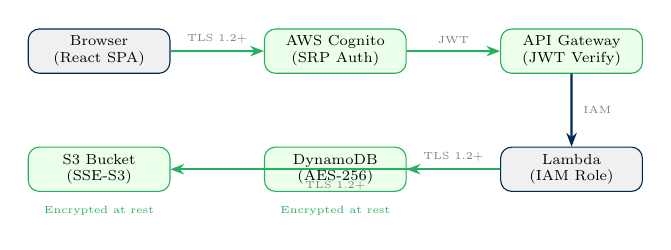
\begin{tikzpicture}[scale=0.75, transform shape,
  box/.style={rectangle, rounded corners=4pt, draw=UNBBlue, fill=UNBLightGray, minimum width=2.4cm, minimum height=0.75cm, font=\scriptsize, align=center},
  secure/.style={rectangle, rounded corners=4pt, draw=UNBGreen, fill=green!8, minimum width=2.4cm, minimum height=0.75cm, font=\scriptsize, align=center},
  arrow/.style={-{Stealth[length=5pt]}, thick, UNBBlue},
  sarrow/.style={-{Stealth[length=5pt]}, thick, UNBGreen},
  label/.style={font=\tiny, UNBGray, midway, above}
]

\node[box] (browser) at (0,3) {Browser\\(React SPA)};
\node[secure] (cognito) at (4,3) {AWS Cognito\\(SRP Auth)};
\node[secure] (apigw) at (8,3) {API Gateway\\(JWT Verify)};
\node[box] (lambda) at (8,1) {Lambda\\(IAM Role)};
\node[secure] (dynamo) at (4,1) {DynamoDB\\(AES-256)};
\node[secure] (s3) at (0,1) {S3 Bucket\\(SSE-S3)};

\draw[sarrow] (browser) -- node[label] {TLS 1.2+} (cognito);
\draw[sarrow] (cognito) -- node[label] {JWT} (apigw);
\draw[arrow] (apigw) -- node[label, right, xshift=2pt] {IAM} (lambda);
\draw[sarrow] (lambda) -- node[label] {TLS 1.2+} (dynamo);
\draw[sarrow] (lambda) -- node[label, below, yshift=-2pt] {TLS 1.2+} (s3);

% Encryption labels
\node[font=\tiny, UNBGreen] at (4,0.3) {Encrypted at rest};
\node[font=\tiny, UNBGreen] at (0,0.3) {Encrypted at rest};

\end{tikzpicture}

\vspace{0.5em}
{\small Every communication path is encrypted in transit (TLS 1.2+). All data stores use AES-256 encryption at rest. Authentication uses Cognito SRP protocol --- passwords never transmitted.}
\end{frame}

\end{document}
